\documentclass[12pt]{article}
\usepackage{geometry}                % See geometry.pdf to learn the layout options. There are lots.
\geometry{a4paper}    
\usepackage[german]{babel}               
\usepackage{graphicx}
\usepackage{amssymb}
\usepackage{amsthm}
\usepackage{epstopdf}
\usepackage[utf8]{inputenc}
\usepackage[usenames,dvipsnames]{color}
\usepackage[table]{xcolor}
\usepackage{hyperref}
\usepackage{eurosym}

\DeclareGraphicsRule{.tif}{png}{.png}{`convert #1 `dirname #1`/`basename #1 .tif`.png}

\theoremstyle{definition}
\newtheorem{example}{Example}

\newenvironment{explanation}{%
   \setlength{\parindent}{24pt}
   \itshape
   \color{blue}
}{}

%Dies kann -und sollte bei der Ausgangssituation anstelle der doppelten Backslashes verwendet werden! -MH
\newcommand*{\skippingparagraph}{\par\vspace{\baselineskip}\noindent}

\newcommand{\projectname}{ReceiptManager}
\newcommand{\productname}{ReceiptManager}
\newcommand{\projectleader}{J. Richtsfeld}
\newcommand{\documentstatus}{In Arbeit}
\newcommand{\appname}{Dinly }
\newcommand{\version}{V. 1.0}

\begin{document}
\begin{titlepage}
\begin{flushright}

\includegraphics[scale=.5]{htlleondinglogo.png}
\end{flushright}



\vspace{10em}

\begin{center}
{\Huge Projektantrag} \\[3em]
{\LARGE \productname} \\[3em]
\end{center}

\begin{flushleft}
\begin{tabular}{|l|l|}
\hline
Projekt Name & \projectname \\ \hline
Projekt Leiter & \projectleader \\ \hline
Dokumenten Status & \documentstatus \\ \hline
Version & \version \\ \hline
\end{tabular}
\end{flushleft}

\end{titlepage}
\section*{Revisions}
\begin{tabular}{|l|l|l|}
\hline
\cellcolor[gray]{0.5}\textcolor{white}{Date} & \cellcolor[gray]{0.5}\textcolor{white}{Author} & \cellcolor[gray]{0.5}\textcolor{white}{Change} \\ \hline
16.09.2019&J.R./G.R./M.H./M.K.&Erste version \\ \hline
20.09.2019&J.R./G.R./M.H./M.K.&Projektziele überarbeitet \\ \hline
23.09.2019&J.R./G.R./M.H./M.K.&Rechtliches und Rahmenbedingungen \\ \hline
27.09.2019&J.R./G.R./M.H./M.K.&Projektantrag Korrektur und Finalisierung \\ \hline
7.10.2019&J.R./G.R./M.H./M.K.&Erweiterung und Verbesserung der Ausgangssituation \\ \hline
14.10.2019&J.R./G.R./M.H./M.K.&Skizzen erstellt und hinzugefügt \\ \hline
21.10.2019&J.R./G.R./M.H./M.K.&Korrekturen und Anpassungen an Skizzen\\ \hline
25.10.2019&J.R./G.R./M.H./M.K.&Finalisierung des Kompletten Dokuments\\ \hline
\end{tabular}
\pagebreak
\tableofcontents
\pagebreak

\section{Einleitung}

\appname soll den Nutzern mit geringem Aufwand eine ausgewogene Ernährung ermöglichen. Dafür wird ein individueller Ernährungsplan erstellt, der auf den Daten des Benutzers basiert (zb. Gewicht, Größe, Ernährungsgewohnheiten, Allergien, Nahrungsunverträglichkeiten, etc.). Auf Basis dieses Ernährungsplans werden Rezepte zum selber kochen oder bestellen vorgeschlagen. Die benötigten Zutaten können direkt über die App bestellt werden und werden im geplanten Zeitrahmen an die Kunden geliefert (Kooperation mit Lebensmittlelkonzernen z.B.: Rewe, Spar) . Außerdem besteht die Möglichkeit sich direkt über die App fertige Gericht liefern zu lassen (Kooperation mit Lieferdiensten: Lieferando, Mjam). Des Weiteren wird durch einen Kalorientracker, die tägliche Kalorienaufnahme überwacht um eine optimale Ernährung zu gewährleisten.
\pagebreak

\section{Ausgangssituation}

Die Ernährung in der westlichen Welt wird immer schlechter. Die Bevölkerung möchte tendenziell weniger Zeit für die Planung und Zubereitung von Mahlzeiten aufwenden. Da oft keine Ideen für neue Speisen vorhanden sind, wird die Ernährung schnell eintönig und unausgewogen. Betreibt man zusätzlich noch Sport und möchte seine Kalorienzufuhr überwachen, so ist dies sehr Aufwendig, da jeder Bestandteil einer Mahlzeit manuell eingegeben werden muss. Dazu kommt, dass man seine Lebensmitteleinkäufe gut planen muss um Abfälle zu vermeiden und Geld zu sparen.

Kokurrenz

Unser Ansatzpunkt


\section{Allgemeine Bedinungen und Einschränkungen}
Unsere App muss mit folgenden Problemen umgehen können:

\baselineskip Da das bevorzugtes Essen einer Person je nach Region variiert, muss unser System auf der beim Registrierungsprozess eingegebenen Daten, passende Rezepte/Gerichte vorschlagen.

Der Ernährungsplan/Die ausgesuchten Gerichte müssen optimal auf den Geschmack des Kunden abgestimmt sein, um den Kunden an die App zu binden.

Beim Registrierungsprozess werden viele sehr sensible Daten angegeben, daher müssen die Daten sicher gespeichert werden.

Der Benutzer muss durch eine Variation von Lebensmitteln, die durch Bilder graphisch veranschaulicht sind (welche dem Nutzer eigentlich nur als Inspirierung dienen sollen) unterhalten werden und zeitlich an die App gebunden werden.


\section{Projektziele und Systemkonzepte}
Die Projektziele werden wie folgt zusammengefasst:

\subsection{Benutzeroberfläche Steuerberater}


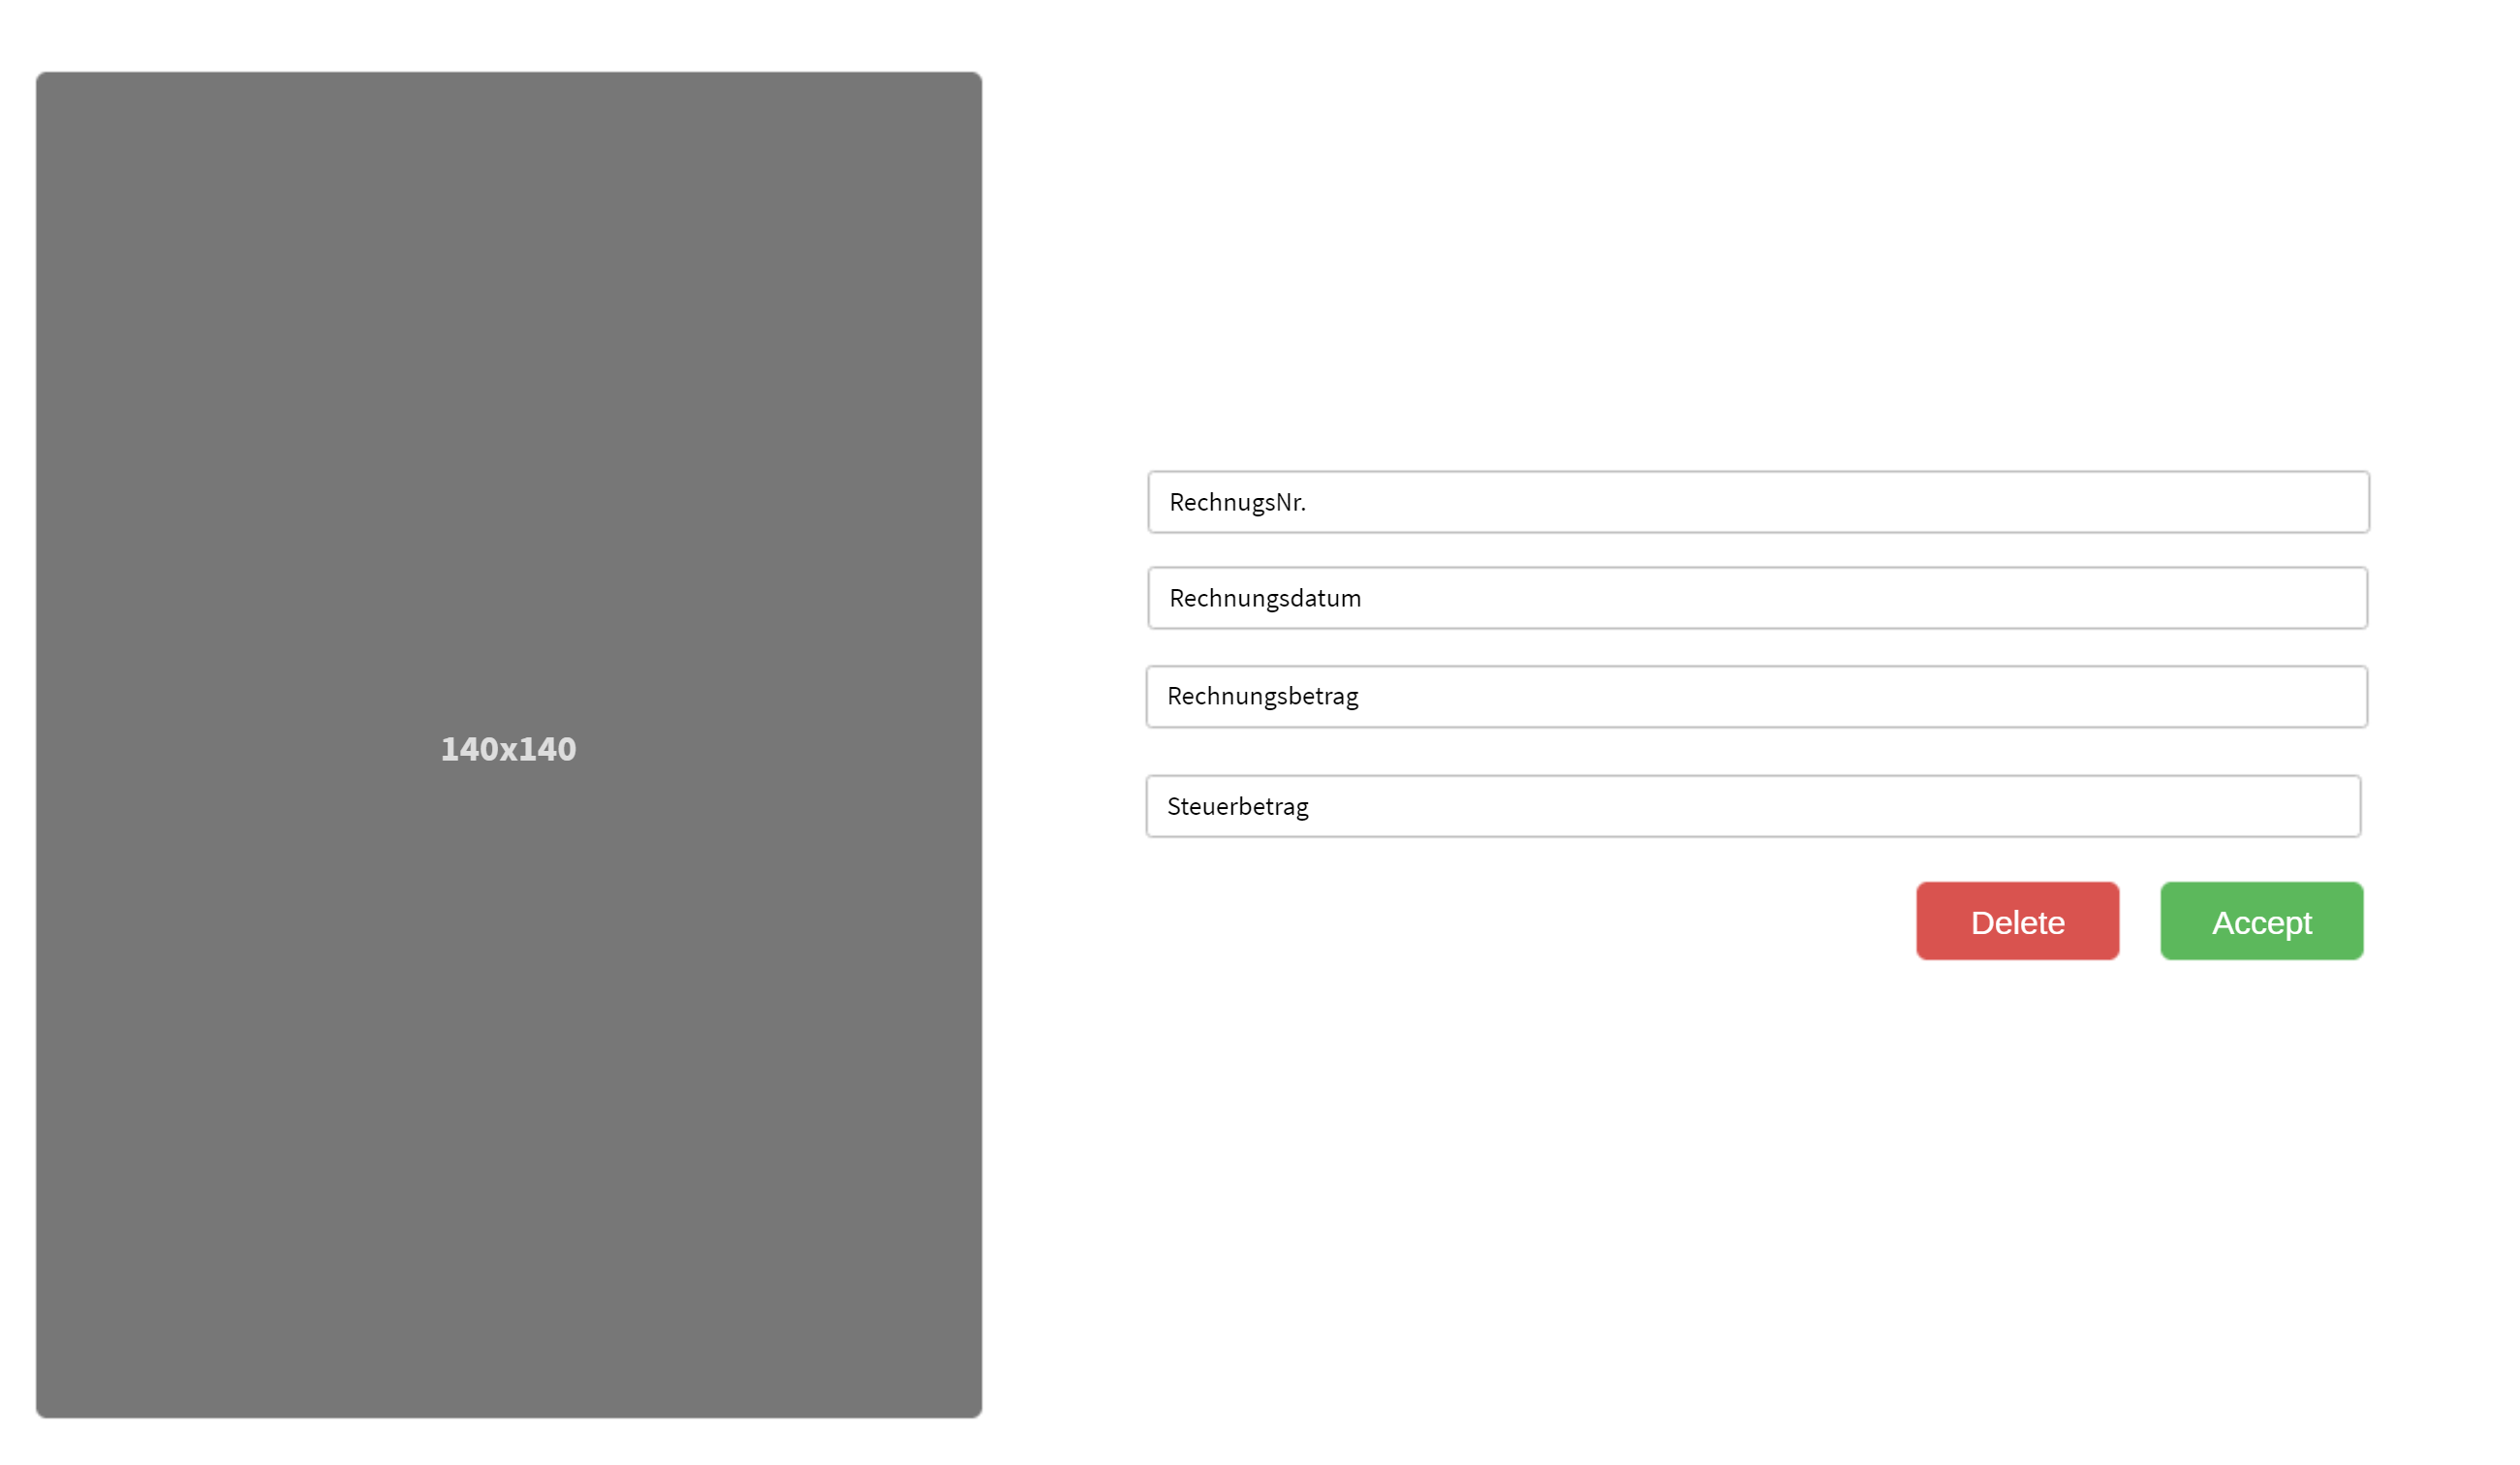
\includegraphics[width=\linewidth]{SingleReceiptReview}

\noindent Innerhalb eines Jahres können die Rechnungen nach Datum und Betrag sortiert werden, um dem Steuerberater das Suchen der Rechnungen/Belege möglichst einfach und schnell zu gestalten.
\par

\pagebreak
\subsection{Benutzeroberfläche Klient}
Ein großer Fokus liegt bei dem Projekt auf einer Mobilapp für den Klienten. Die Kamera und kompakte Bauart eines Smartphones ermöglicht schnelle Schnappschüsse und benötigt keinen Scanner.

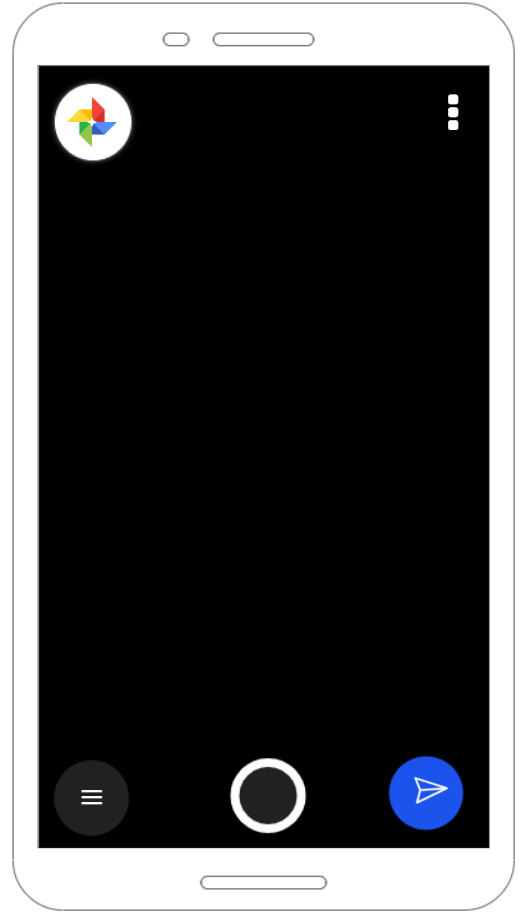
\includegraphics[scale=0.5]{MobileSnapshotReceiptConcept}

\pagebreak
\subsection{Backend}
Das Backend soll auf zwei Teile aufgeteilt werden. Zum einen das OCR- System als Microservice und zum anderen das Hauptbackend zum Speichern und Verwalten der Belege.
\skippingparagraph
Beim Frontend wird für die Klienten eine Web App bzw. Mobileapp angeboten. Der Steuerberater sieht die Admin-Oberfläche nur in der Webapp da, kein Bedarf besteht dies in einer Mobileapp zu realisieren.

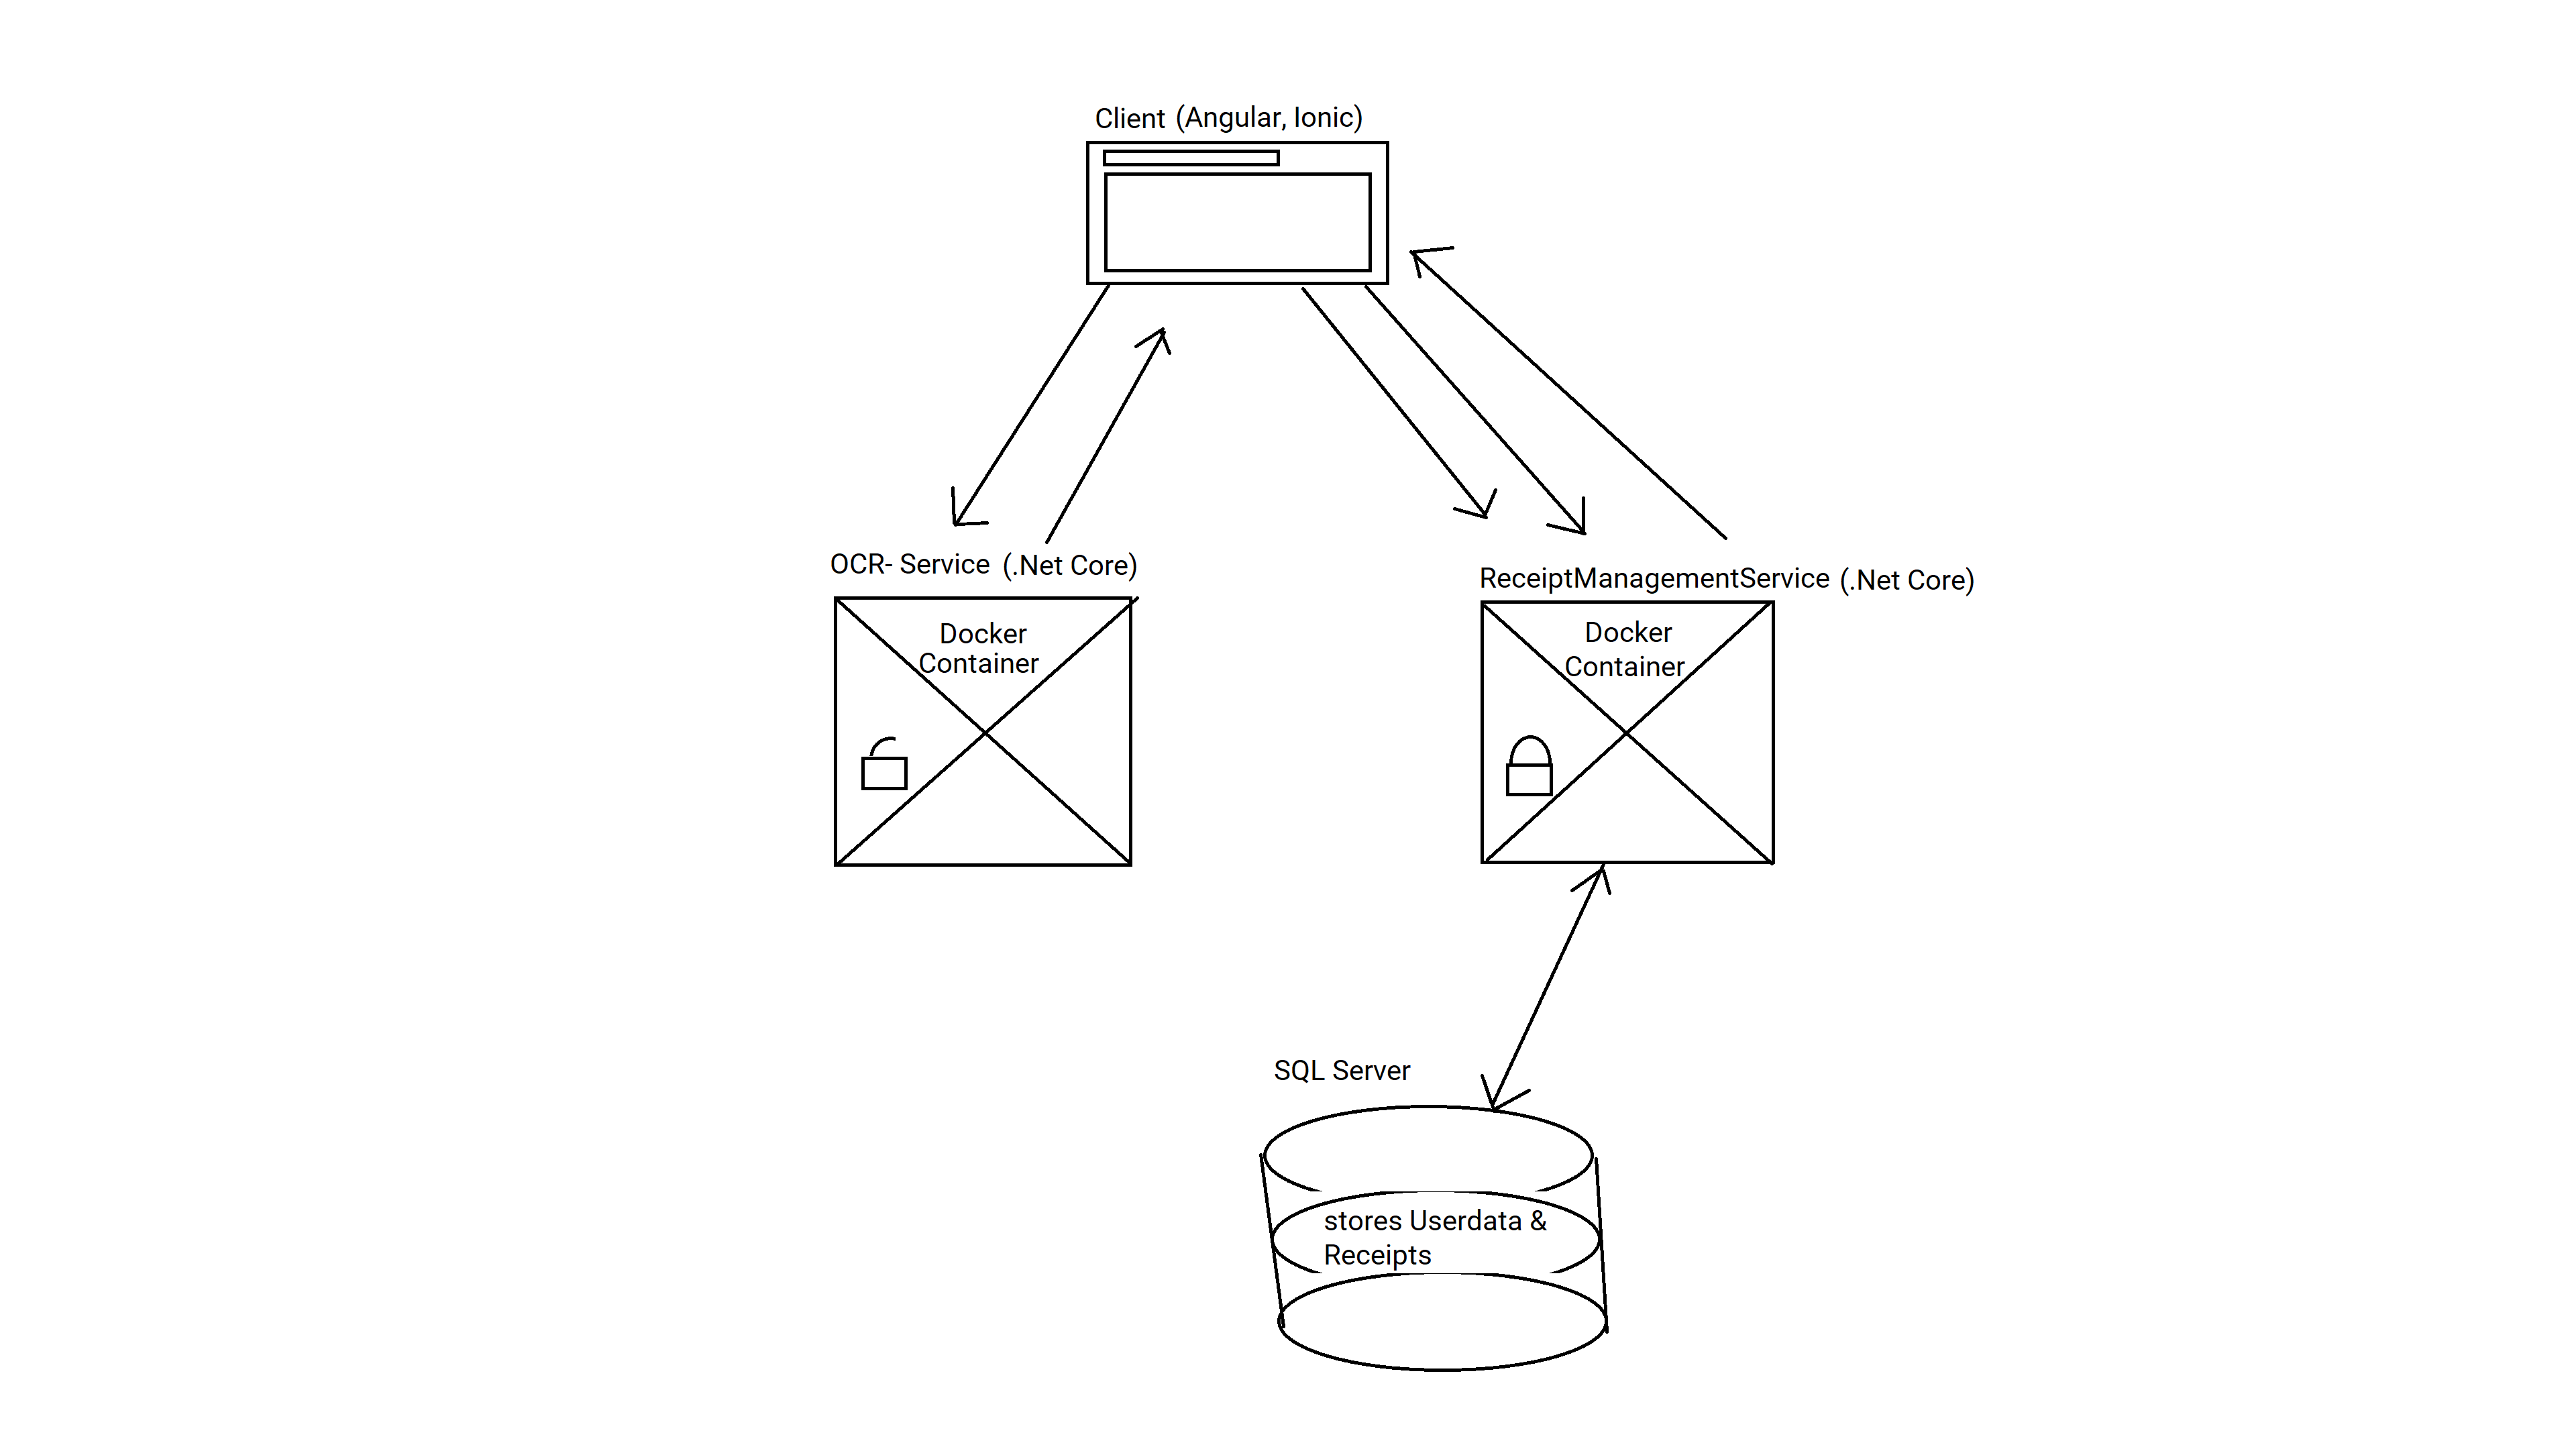
\includegraphics[width=\linewidth,trim=130mm 10mm 100mm 10mm, clip]{SystemConcept}
\pagebreak


\section{Chancen und Risken}

\subsection{Vorteile und Chancen durch und von unsere Software}

Der Klient kann sich durch unsere Software Zeit und daher Geld sparen, da er keine Zeit mehr verschwenden muss, um die Rechnungen bei sich in Ordner einzusortieren und diese dann zum Steuerberater zu bringen.\\ \\
Die Verwaltung der Rechnungen wird einfacher und übersichtlicher, da das Suchen der Rechnungen in Ordner wegfällt und durch einfaches und schnelles Suchen in unserer Anwendung ersetzt wird.\\ \\
Ein großer Vorteil ist die Ersparniss vom Arbeitszeit, da ein Buchhalter etwa 20 Prozent seiner Zeit mit dem Verwalten und Auslesen von Rechnungen verbringt. Bei einem Brutto-Monatsgehalt von \EUR{3000}, werden im Jahr etwa \EUR{8000} und im Monat \EUR{600} pro Mitarbeiter eingespart. Außerdem steigert unsere Anwendung die Produktivität der Buchhalter da sie sich nicht mehr mit den stupiden Arbeiten der Verwaltung auseinander setzen müssen.\\



\subsection{Risiken unserer Software}

Folgende Risiken müssen beachtet werden:
\begin{itemize}
\item Verlust von Belegen, die sensible Informationen enthalten, da es beim Übertragen der Daten zu Fehlern kommen kann.
\item Durch falsch eingegebene von Informationen durch den Steuerberater, könnten inkonsistente Datenbestände entstehen.
\end{itemize}

\pagebreak

\section{Planung}

\subsection{Teammitglieder}

\begin{itemize}
\item Teamleiter: Julian Richtsfeld
\item Entwickler für Benutzeroberfläche: Maximilian Kaindl
\item Entwickler für Web- und Mobilklienten: Matthias Hofmarcher
\item Entwickler für OCR- und Parsercontainer für automatische Beleginformationserkennung: Gregor Rechberger
\item Entwickler für Backend: Julian Richtsfeld
\end{itemize}

\subsection{Meilensteine}

\begin{tabular}{|l|l|}
\hline
\cellcolor[gray]{0.5}\textcolor{white}{Date} & \cellcolor[gray]{0.5}\textcolor{white}{Meilenstein} \\ \hline
20.12.2019&Authentifizierung mit JSON-Webtoken und Identity Server 4\\ \hline
28.02.2020&Server Prototyp als Api-Endpunkt lauffähig \\ \hline
03.04.2020&Web-Client Prototyp lauffähig \\ \hline
24.04.2020&OCR-Prototyp abgeschlossen \\ \hline
29.05.2020&Mobile-Client-Prototyp lauffähig\\ \hline
26.06.2020&Lauffähiger Receipt-Manager Prototyp\\ \hline
\end{tabular}

\subsection{Benoetigte Ressourcen}

\begin{itemize}
\item Server (Eigenbau oder Cloud)
\item OCR-Software Lizenz
\end{itemize}

\subsection{Projektdauer}
Das Projekt beginnt mit 20.09.2019 und endet mit dem Ende des Schuljahres 2019/20. Der erste Prototyp wird Mitte November zur Verfuegung stehen. Die Implementierung beginnt mit Abschluss des Prototyps. Die groeßeren Arbeitspakete sind die Entwicklungs des Front -und Backends und die Einbindung einer OCR-Software. Unsere Ziele schaetzen wir durchaus realistisch ein und gehen von einer fristgerechten Umsetzung aus.

\end{document}  